\section{Pre-processing}\label{LocatingCenter}

A number of pre-processing steps are required before running any kind of modelfitting process on a frame.
Several pieces of information are gathered:

\begin{enumerate}
	\item The greatest z value for a filled voxel.
		This is used to determine the height of the figure.
		Half this height is assumed to be the height of the hips.
	\item The mean coordinate.
		This is taken to represent the center of the figure and is used to normalise his position as he walks across the frame.
		It is calculated as follows:
		\begin{equation}
			\mathbf{V}_{mean} = (\overline{x}, \overline{y})
		\end{equation}
		Where
		\begin{align}
			\overline{x} &= \frac{1}{s_x s_y s_z} \sum_{x=1}^{s_x} \sum_{y=1}^{s_y} \sum_{z=1}^{s_z} x I(x,y,z) \\
			\overline{y} &= \frac{1}{s_x s_y s_z} \sum_{x=1}^{s_x} \sum_{y=1}^{s_y} \sum_{z=1}^{s_z} y I(x,y,z)
		\end{align}
\end{enumerate}

The key assumption made here is that a subject's legs ``start'' half way between his feet and the top of his head.
Figure \ref{Preprocessing} demonstrates this by showing how the greatest z value for a filled voxel, $h$, is used to
indicate the starting position of the legs.
TODO: check if this is generally right.

\begin{figure}[b]
	\centering
	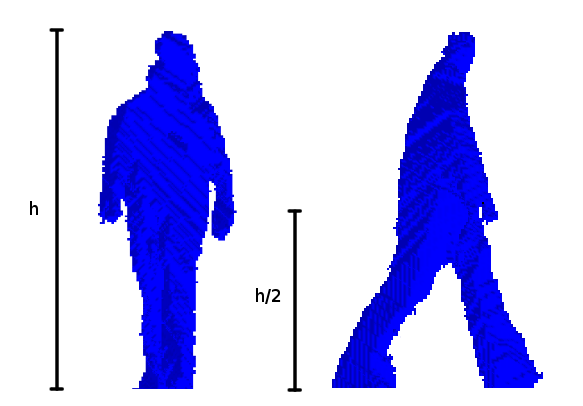
\includegraphics[height=6cm]{preprocessing.png}
	\caption{The information gathered during the pre-processing step is used as a guide for where to start searching for the legs.}
	\label{Preprocessing}
\end{figure}
